\documentclass[a4paper, 12pt]{article}
\usepackage[left = 13 mm, top = 15mm, right = 13 mm, bottom = 18mm, bindingoffset = 7mm]{geometry}
\usepackage[T2A,T1]{fontenc}
\usepackage[utf8]{inputenc}
\usepackage[english,russian]{babel}
\usepackage{graphicx}
\usepackage{amssymb, mathtools}
\usepackage[normalem]{ulem}
\useunder{\uline}{\ul}{}
\usepackage{lipsum}
\usepackage{float}
\usepackage{wrapfig}
\usepackage{indentfirst} 

\newcommand{\HRule}{\rule{\linewidth}{0.3mm}}
\newcommand{\LabTitle}{Магнетометр}
\begin{document}




\begin{titlepage}
\begin{center}\large
ФГАУ ВПО <<МОСКОВСКИЙ ФИЗИКО-ТЕХНИЧЕСКИЙ УНИВЕРСИТЕТ>>
\begin{figure}[H]
\centering

\includegraphics[width=15cm]{logo.jpg}
\end{figure}
{\Large
Кафедра радиотехники}

\vfill

\hrule
\vspace{0.3cm}

\huge \LabTitle

\vspace{0.3cm}
\hrule


%\noindent\rule{\textwidth}{0.4mm}
%\huge Магнитометр
%\noindent\rule{\textwidth}{0.4mm}


\end{center}

\vfill


\begin{minipage}{0.7\textwidth}
\textbf{Выполнил:}
Корепанов Г.М.

512 группа

\vspace{0.5cm}

\textbf{Преподаватель:}
Филатов Иван Васильевич
\end{minipage}


\vfill
\centering
 Долгопрудный, 2016 г.




\end{titlepage}


\section*{Теоретические выкладки}
\subsection*{Вектор-потенциал МП, созданного системой стационарных токов}
{
Закон Био-Савара-Лапласа может считаться обобщением множества экспериментальных фактов (хотя может быть выведен из уравнений Максвелла, что идейно отражает то же самое, ведь уравнения Максвелла сами по сути являются обобщением эксп. фактов):

$$ d\vec B=\frac{1}{c}\frac{[\vec j(\vec{r_1}), (\vec{r}-\vec{r_1})]}{|\vec{r} - \vec{r_1}|} dV_1.$$

Используя математические тождества 

$$ \frac{\vec r - \vec r_1}{|\vec r - \vec r_1|^3}=-\nabla\left(\frac{1}{|\vec r - \vec r_1|}\right),$$

$$[\vec a, \nabla \varphi]=-\operatorname{rot}(\vec a \varphi),$$
где вектора $\vec a$ и $\vec r_1$ полагаются константами, получим выражение

$$d \vec B(\vec r) = \frac{1}{c}\operatorname{rot}\left(\frac{\vec j (\vec r_1)}{| \vec r - \vec r_1 |} \right) d V_1.$$

Элементарное интегрирование по всем элементам тока даёт выражение для полной величины напряженности магнитного поля в точке:

$$ \vec B(\vec r) = \frac{1}{c}\operatorname{rot}\int\limits_{V} \frac{\vec j (\vec r_1)}{| \vec r - \vec r_1 |}  d V_1.$$

Получили явное выражение для векторного потенциала МП, созданного постоянным распределением токов:

$$ \vec A (\vec r) = \frac{1}{c}\int\limits_{V} \frac{\vec j (\vec r_1)}{| \vec r - \vec r_1 |}  d V_1,$$

\begin{equation}
\label{b=rota}
\vec B = \operatorname{rot} \vec A.
\end{equation}

Если движущиеся заряды распределены дискретно, то формула принимает вид
$$ \vec A (\vec r) = \frac{1}{c}\sum\limits_{i} \frac{q_i \vec \nu_i}{| \vec r - \vec r_i |} .$$

}

\subsection*{Поле магнитного диполя}
{

Используем полученный результат для вычисления поля системы токов на большом расстоянии от этой системы.

Учитывая, что для стационарной системы токов $\sum\limits_{i} q_i \vec \nu_i \simeq 0 $, и, в силу удалённости системы токов ($ r \gg r_i \hspace{5pt}\forall i$), получим приближённое выражение для векторного потенциала МП:

$$\vec A = \frac{[\vec m, \vec r]}{r^3},$$
где $\vec m$ -- стандартное обозначение магнитного момента системы токов:

$$\vec m = \frac{1}{2c}\sum\limits_{i} q_i[\vec r_i, \vec \nu_i].$$ 

Магнитное поле найдём из (\ref{b=rota}):

$$ \vec B = \frac{3(\vec m \vec r)\vec r - \vec m r^2}{r^5}$$

Отсюда сразу следует, что поле магнитного стержня с магнитным моментом $\vec m$ на перпендикуляре к стержню 

$$B(r_\perp) = \frac{m}{r^3}.$$
}

\section{Измерение горизонтальной составляющей поля Земли}
\section*{Расчётные формулы}
Поле диполя на расстоянии $R$ от него на перпендикуляре к нему:
\begin{equation}
B_\perp = \frac{m}{R^3}  \quad \text{СИ: } B_\perp=\frac{\mu_0}{4\pi}\frac{m}{R^3}
\end{equation}

Поле в центре многовиткового кольца с током с радиусом $R$ и количеством витков $N$ ищется интегрированием закона Био-Савара-Лапласа:
\begin{equation}\label{circlecurrent}
B_I=\frac{2\pi}{c}\frac{I}{R}N, \quad \text{СИ: } B_I=\frac{\mu_0}{2}\frac{I}{R}N
\end{equation}


Угол отклонения стрелки связывает и искусственное МП, созданное диполем, и поле Земли $B_0$:
$$ \frac{B_{\perp}}{B_0} = \tg{\varphi},\quad \tg{\varphi} = \frac{x}{2L}$$
Получить дополнительное уравнение на магнитный момент стержня легко, определив период его крутильных колебаний в поле Земли:

\begin{equation}\label{period}
T = 2\pi\sqrt{\frac{J}{mB_0}},
\end{equation}

где $J$ -- момент инерции стержня, который можно рассчитать непосредственно из его массы и геометрии:
\begin{equation}\label{inertia}
J=m\left(\frac{l^2}{12}+\frac{r^2}{4}\right).
\end{equation}


Объединяя используемые формулы, получим окончательную, расчётную
\begin{equation}
B_0 = \frac{\sqrt{2\pi}}{TR}\sqrt{\frac{\mu_0JL}{Rx}},
\end{equation}

в которую входят экспериментально измеряемые величины\\
$x$ -- смещение светового зайчика,\\
$L$ -- расстояние от шкалы до зеркальца,\\
$R$ -- радиус кольца,\\
$T$ -- период колебаний (\ref{period}),\\
$J$ -- момент инерции стержня, рассчитываемый по его параметрам (\ref{inertia}).

\section*{Экспериментальная установка}

\begin{figure}[H]
\centering
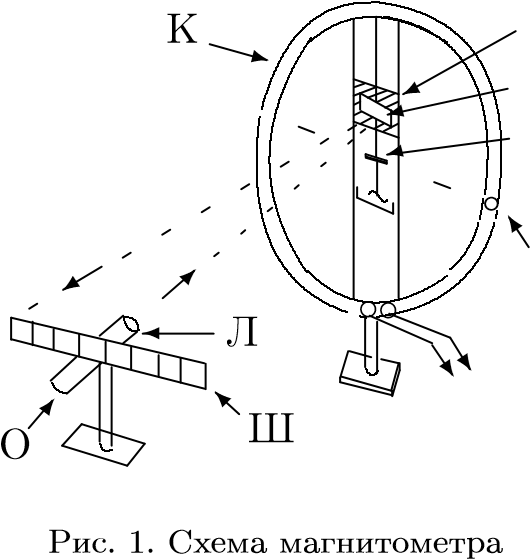
\includegraphics[scale=0.5]{1}
\caption{З1, З2 -- настроечные зеркала, К -- контур с намоткой из провода, О -- осветительная лампа, Ш -- отсчётная шкала.}
\end{figure}

\section*{Экспериментальные данные}
\subsection*{Колебания стержня}
\begin{table}[H]
\centering


\begin{tabular}{|l|l|l|l|}
\hline
\textbf{№} & \textbf{$\mathbf{t}$, с} & \textbf{$\mathbf{N}$, раз} & \textbf{$\mathbf{T}$, с} \\ \hline
\textbf{1} & 293,09          & 30                & 9,8             \\ \hline
\textbf{2} & 182,78          & 20                & 9,1             \\ \hline
\textbf{3} & 231,36          & 25                & 9,3             \\ \hline
\textbf{4} & 236,92          & 25                & 9,5             \\ \hline
\end{tabular}
\caption{Колебания стержня в поле земли при разных длинах подвеса}


\end{table}

С приемлемой точностью упругость нити не влияет на период колебаний стрежня в МП:

$$T = (9,4\pm0,4) \text{ с}$$


\subsection*{Смещение зайчика при приближении диполя}

\begin{table}[H]
\centering
\begin{tabular}{|l|l|l|}
\hline
\textbf{№}          & \textbf{$\mathbf{x_\leftarrow}$, мм} & \textbf{$\mathbf{x_\rightarrow}$, мм} \\ \hline
\textbf{1} & 166                         & 155                          \\ \hline
\textbf{2} & 161                         & 170                          \\ \hline
\textbf{3} & 164                         & 166                          \\ \hline
\end{tabular}
\caption{Смещение светового зайчика при внесении диполя}

\end{table}

Среднее значение смещения:

$$x = (165\pm4) \text{ мм}$$

\subsection*{Геометрические параметры установки и диполя}
\subsubsection*{Установка:}
$$L = (115,5\pm0.5) \text{ см -- расстояние до зеркала}$$
$$R = (20\pm0,2) \text{ см -- радиус кольца}$$
\subsubsection*{Диполь:}
$$r = (5,42\pm0,01) \text{ мм}$$
$$l = (39,90\pm0,05) \text{ мм}$$
$$m = (5,880) \text{ гр}$$

\section*{Результаты}
Момент инерции стержня из (\ref{inertia}):
$$ J = (823\pm5) \text{ г}\cdot\text{мм}^2$$

Магнитное поле Земли:
$$ B_0 = (8,0\pm0,7)\text{ мкТл.}$$


\section{Определение электродинамической постоянной ($\mathbf c$)}
Аналогично предыдущим измерениям, определим ток, протекающий по кольцу, по углу отклонения стрелки. Используя формулу (\ref{circlecurrent}), и зная теперь значение магнитного поля Земли в точке нахождения установки, можно вычислить ток, протекающий по кольцу (в единицах СИ):
$$I_\text{СИ}=\frac{B_0 R}{\mu_0 N L} \cdot x.$$

Одновременно тот же ток можно измерить из других соображений. Используя электромагнитное реле, можно периодически заряжать конденсатор и разряжать его на кольце. Емкость конденсатора должна быть достаточно мала, чтобы он успевал полностью разряжаться за время переключения реле.

$$I_\text{СГС}=CUn.$$
$$[U]_\text{СГС}\simeq300^{-1}[U]_\text{СИ}.$$



\section*{Экспериментальные данные}

\subsection*{Смещение зайчика при приближении диполя}

\begin{table}[H]
\centering
\begin{tabular}{|l|l|l|}
\hline
\textbf{№}          & \textbf{$\mathbf{x_\leftarrow}$, мм} & \textbf{$\mathbf{x_\rightarrow}$, мм} \\ \hline
\textbf{1} & 199                         & 197                          \\ \hline
\textbf{2} & 203                         & 204                          \\ \hline
\textbf{3} & 200                         & 199                          \\ \hline
\end{tabular}
\caption{Смещение светового зайчика при включении реле}
\end{table}

Среднее значение смещения:
$$x = (200\pm2) \text{ мм}$$
\subsection*{Параметры установки}
$$C=9\cdot 10^5 \text{ см } (\varepsilon_C = 2\%)$$
$$n = 50 \text{ Гц}$$
$$N = 44 \text{ витка}$$
$$U=95,5\pm 0,5 \text{ В}$$

\section*{Результаты}
$$I_\text{СИ} = (5,0\pm0,5) \text{ мА}$$
$$I_\text{СГС}= (14,3\pm0,33)\cdot10^{6} \text{ ед. СГС}$$

$$c=\frac{1}{10}\frac{I_\text{СГС}}{I_\text{СИ}}\cdot\frac{\text{м}}{\text{с}} = 2,86\cdot 10^8\ \frac{\text{м}}{\text{с}}$$

\section*{Выводы}
Были получены удовлетворительные результаты, с хорошей точностью воспроизводящие известные данные. Изучены основные особенности систем СИ и СГС, простейшие вопросы магнитостатики.

\end{document}